% Template for CAD in medical imaging - Project Report
%          spconf.sty  - ICASSP/ICIP LaTeX style file, and
%          IEEEbib.bst - IEEE bibliography style file.
% --------------------------------------------------------------------------
\documentclass{article}
\usepackage{spconf,amsmath,graphicx}
\usepackage{subfigure}

% Title
\title{Computer Aided Diagnosis\\LUNA16: Candidate detection}
%
\makeatletter
\def\@name{ \emph{Luc Nies (s4136748)}, \emph{Tom van de Poll (s4106512)}, \emph{Harmen Prins (s4132297)}, \\ \emph{Steven Reitsma (s4132343)} \& \emph{Inez Wijnands (s4149696)}}
\makeatother

\address{Radboud University Nijmegen}
%
% For example:
% ------------
%\address{School\\
%	Department\\
%	Address}
%
% Two addresses (uncomment and modify for two-address case).
% ----------------------------------------------------------
%\twoauthors
%  {A. Author-one, B. Author-two\sthanks{Thanks to XYZ agency for funding.}}
%	{School A-B\\
%	Department A-B\\
%	Address A-B}
%  {C. Author-three, D. Author-four\sthanks{The fourth author performed the work
%	while at ...}}
%	{School C-D\\
%	Department C-D\\
%	Address C-D}
%
% More than two addresses
% -----------------------
% \name{Author Name$^{\star \dagger}$ \qquad Author Name$^{\star}$ \qquad Author Name$^{\dagger}$}
%
% \address{$^{\star}$ Affiliation Number One \\
%     $^{\dagger}$}Affiliation Number Two
%
\begin{document}
%\ninept
%
\maketitle
%
\begin{abstract}
Write your abstract here.
\end{abstract}


% Introduction
\section{Introduction}
\label{sec:intro}
In the \emph{LUng Nodule Analysis 2016 (LUNA16)} challenge, we aim to detect lung nodules in low-dose lung CT images. Firstly, we have segmented the lungs from the images. The next step is identifying candidates for lung nodules. Our aim is to detect enough candidates to include all actual lung nodules. In other words, be as sensitive as possible. The future step is of course to remove the false positives, but first we strive towards including the annotated nodules.

We continued working on the deep learning approach we used for the previous phase. In that phase we worked on lung segmentation and for this phase we treated candidate detection again as a segmentation problem. Secondly, we also used an image processing approach where we use the features of nodules such as blobness for candidate detection. These approaches and results are explained more detailed in the following sections.

% Table
\begin{table}[h]
\caption{\small{Caption here.}}
\label{tab:parameters}
\centering
\begin{tabular}{c | c | l}
text & text & text\\
\hline \hline
text & text & text
\end{tabular}
\end{table}

You can include figures as follows:

% Figure
\begin{figure}[h]
\centering
\subfigure[]
{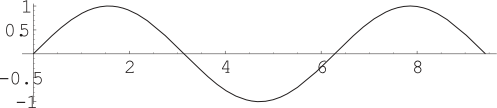
\includegraphics[width=0.7\linewidth]{./figure.png}}
\subfigure[]
{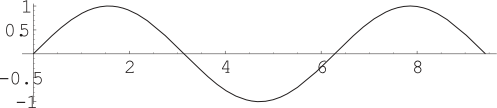
\includegraphics[width=0.7\linewidth]{./figure.png}}
\caption{Caption here. \label{figure:patterns}}
\end{figure}

% Method
\section{Method}\label{sec:method}
Explain the proposed method here.
You can use subsections to detail each part of your approach as follows. 
\subsection{Fully convolutional network}
Your text here.

\subsection{Nodule detection using blobness feature}
We used a second approach for detection lung nodule candidates which is the more conventional approach of using their blob-like structure. The first step is applying the lung segmentation as a mask on the lung CT images to reduce the search space to the actual lungs. The algorithm for the actual candidate detection is as follows:

\begin{itemize}
\item Apply two different sized Laplacian of Gaussian (LoG) filters. A LoG filter is circular-symmetric and thus widely used for blob detection, but has a maximum response to a particular blob size. We combined two filters with normalized kernels (IS THIS NORMALIZED?), the first with $\sigma = 3$ and \emph{kernel extent} = 7 and the second with $\sigma = 5$ and \emph{kernel extent} = 11 CHECK VALUES. We chose these parameters based on the paper of Van de Leemput et al. \cite{leemput}
\item Take the pixel-wise maximum of the results of the LoGs to combine them to one result.
\item Threshold the resulting image with value THRESHOLDVALUEAFTERLOGS. See Figure \ref{figure:LoGresult} for an example result. This value is established by sampling the values of known nodules and healthy lung tissue.
\begin{figure}[h]
\centering
{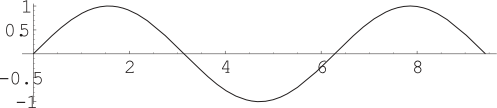
\includegraphics[width=0.7\linewidth]{./figure.png}}
\caption{The thresholded image after taking the maximum of the two LoGs. \label{figure:LoGresult}}
\end{figure}
\item Do a connected component analysis on the resulting image, and select only components with values between CONNECTEDCOMPONENTSVOLUMEVALUES. This identifies the initial candidates. See Figure \ref{figure:conncomp} for an example result.
\begin{figure}[h]
\centering
{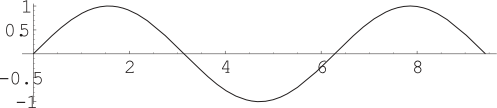
\includegraphics[width=0.7\linewidth]{./figure.png}}
\caption{The result of applying a connected component analysis on the image shown in Figure \ref{figure:LoGresult}. \label{figure:conncomp}}
\end{figure}
\item Threshold the resulting image again with value THRESHOLD2VALUE.
\item Apply a Hough transform to identify unwanted candidates, i.e. candidates with features not corresponding to lung nodule characteristics.
\item Threshold the resulting image again to remove the candidates identified by the Hough transform and keep the lung nodule candidates. See Figure \ref{figure:Houghresult} for an example result.
\begin{figure}[h]
\centering
{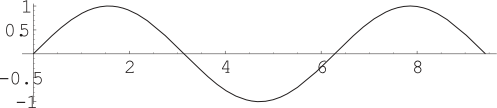
\includegraphics[width=0.7\linewidth]{./figure.png}}
\caption{An example result after applying the Hough transform and thresholding. \label{figure:Houghresult}}
\end{figure}
\end{itemize}
ADD IMAGES

% Experiments
%\section{Experiments}\label{sec:experiments}


% Results
\section{Results}\label{sec:results}
\subsection{Conventional method}
The results are based on the first 30 images in subset 9 of the dataset. The results are evaluated in two ways: the dice score of the predictions to the ground truth candidates given for this phase of the assignment, and the recall between the same datasets. The reason that the results are only examined on 30 images is that this method is very time consuming (over ten minutes per image) and the method was completed relatively close to the deadline.

The average dice score obtained by this method is MEANDICESCORE, with a standard deviation of STDDICESCORE. This score is relatively low, compared to the score reached in the previous phase. However, the main goal of this method is to find all posible nodules. Thus, a large recall value is more important than a large dice score.

The recall obtained with this method is RECALL.

\subsection{fcn}

% Discussion
\section{Discussion}\label{sec:discussion}


\appendix
\section{Contributions}
\textbf{Luc Nies:} \\
\\
\textbf{Tom van de Poll:} \\
\\
\textbf{Harmen Prins:} \\
\\
\textbf{Steven Reitsma:} \\
\\
\textbf{Inez Wijnands:} Contributed to creating the MeVisLab candidate detection method using blob detection. Wrote introduction section and method section on the conventional approach in report.

% References should be produced using the bibtex program from suitable
% BiBTeX files (here: strings, refs, manuals). The IEEEbib.bst bibliography
% style file from IEEE produces unsorted bibliography list.
% -------------------------------------------------------------------------
\bibliographystyle{IEEEbib}

\begin{thebibliography}{}

\bibitem{leemput}
S. van de Leemput, F. Dorssers \& B.E. Bejnordi (2015). A novel spherical shell filter for reducing false positives in automatic detection of pulmonary nodules in thoracic CT scans. \emph{Proceedings SPIE Medical Imaging, 9414}:94142P.
\end{thebibliography}



\end{document}
